\documentclass[11pt]{article}
\usepackage{geometry,marginnote} % Pour passer au format A4
\geometry{hmargin=1cm, vmargin=1cm} % 

% Page et encodage
\usepackage[T1]{fontenc} % Use 8-bit encoding that has 256 glyphs
\usepackage[english,french]{babel} % Français et anglais
\usepackage[utf8]{inputenc} 

\usepackage{lmodern,numprint}
\setlength\parindent{0pt}

% Graphiques
\usepackage{graphicx,float,grffile,units}
\usepackage{tikz,pst-eucl,pst-plot,pstricks,pst-node,pstricks-add,pst-fun,pgfplots} 

% Maths et divers
\usepackage{amsmath,amsfonts,amssymb,amsthm,verbatim}
\usepackage{multicol,enumitem,url,eurosym,gensymb,tabularx}

\DeclareUnicodeCharacter{20AC}{\euro}



% Sections
\usepackage{sectsty} % Allows customizing section commands
\allsectionsfont{\centering \normalfont\scshape}

% Tête et pied de page
\usepackage{fancyhdr} \pagestyle{fancyplain} \fancyhead{} \fancyfoot{}

\renewcommand{\headrulewidth}{0pt} % Remove header underlines
\renewcommand{\footrulewidth}{0pt} % Remove footer underlines

\newcommand{\horrule}[1]{\rule{\linewidth}{#1}} % Create horizontal rule command with 1 argument of height

\newcommand{\Pointilles}[1][3]{%
  \multido{}{#1}{\makebox[\linewidth]{\dotfill}\\[\parskip]
}}

\newtheorem{Definition}{Définition}

\usepackage{siunitx}
\sisetup{
    detect-all,
    output-decimal-marker={,},
    group-minimum-digits = 3,
    group-separator={~},
    number-unit-separator={~},
    inter-unit-product={~}
}

\setlength{\columnseprule}{1pt}

\begin{document}

\textbf{Nom, Prénom :} \hspace{8cm} \textbf{Classe :} \hspace{3cm} \textbf{Date :}\\
\vspace{-0.8cm}
\begin{center}
  \textit{Je n'aime pas le travail, nul ne l'aime ; mais j'aime ce qui est dans le travail l'occasion de se découvrir soi-même.}  - \textbf{Joseph Conrad}
\end{center}
\vspace{-0.8cm}

\subsection*{Définitions}
  \begin{enumerate}
    \item[1.] Nombre négatif : \dotfill \\
    \Pointilles[1]
    \item[2.] Nombres opposés : \dotfill \\
    \Pointilles[1]
  \end{enumerate}

\subsection*{Exercice 1 - Calculer}

\begin{multicols}{3}\noindent
    \begin{enumerate}
        \item $-50 \div \ldots\ldots = -10$
        \item $\ldots\ldots \div \left( -4\right) = -1$
        \item $\ldots\ldots + 4 = -5$
        \item $\ldots\ldots + \left( -10\right) = -1$
        \item $-40 \div 10 = \ldots\ldots$
        \item $-80 \div \ldots\ldots = 10$
        \item $-3 - 3 = \ldots\ldots$
        \item $\ldots\ldots \times 10 = -60$
        \item $9 - 1 = \ldots\ldots$
        \item $-4 \times 6 = \ldots\ldots$
        \item $\ldots\ldots - \left( -1\right) = -8$
        \item $1 \div 1 = \ldots\ldots$
        \item $-1 \times \left( -4\right) = \ldots\ldots$
        \item $-10 - \left( -7\right) = \ldots\ldots$
        \item $\ldots\ldots - 4 = -3$
        \item $-8 + \ldots\ldots = -12$
        \item $2 \times 7 = \ldots\ldots$
        \item $4 \times \left( -10\right) = \ldots\ldots$
        \item $\ldots\ldots + \left( -4\right) = 0$
        \item $6 + \ldots\ldots = 14$
    \end{enumerate}
  \end{multicols}

\subsection*{Exercice 2 - signe d'un produit}

\begin{enumerate}
        \item $50 \times 4$ \dotfill
        \item $9 \times (-6) \times 7$ \dotfill
        \item $-2 \times (-7)$ \dotfill
        \item $4 \times 7 \times (-2) \times 5$ \dotfill
        \item $9 \times 6 \times (-6) \times (-5)$ \dotfill
        \item $-10 \times (-7) \times -1 \times - 4 \times -3 \times 500$ \dotfill
\end{enumerate}

\subsection*{Problèmes}

\begin{minipage}[t]{0.25\textwidth}
  \begin{figure}[H]
    \centering
    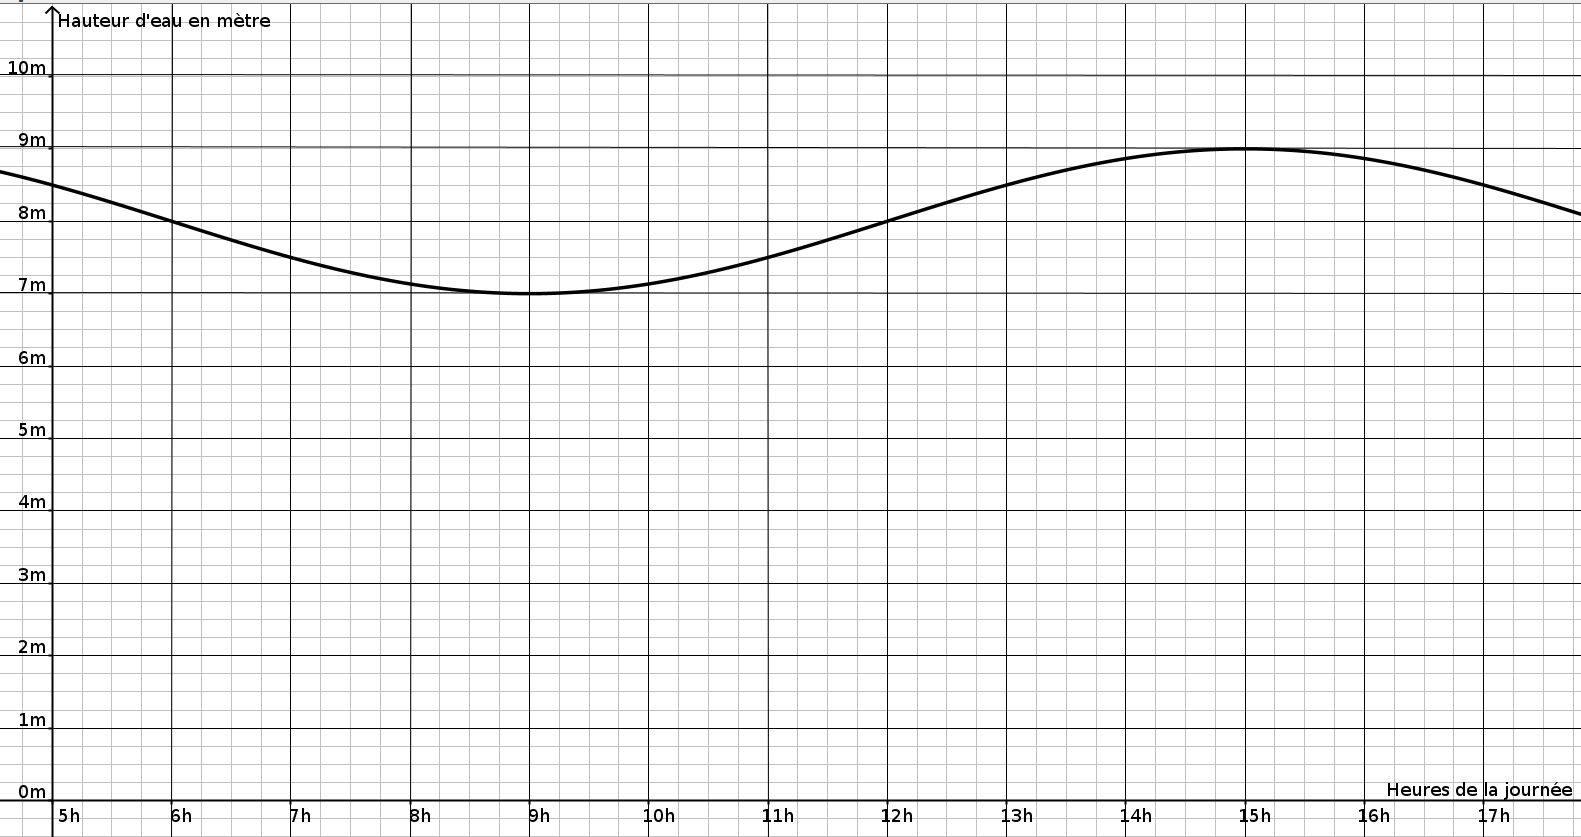
\includegraphics[width=100px]{4x1-relatifs/ex1.jpg}
  \end{figure}
\end{minipage}
\begin{minipage}[t]{0.75\textwidth}
\textbf{1.} Neil Armstrong de l'équipage d'Appolo 11 est sorti du module lunaire le 20 juillet 1969 pour faire le premier pas de l'Homme sur la Lune. La température sur la lune était de $-98 \degree C$. Sa combinaison était chauffée à une température de $18 \degree C$. 

Quelle était la différence de température entre l'intérieur et l'extérieur de sa combinaison ? \\
\Pointilles[6]
\end{minipage}

\begin{minipage}[t]{0.25\textwidth}
  \begin{figure}[H]
    \centering
    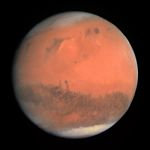
\includegraphics[width=100px]{4x1-relatifs/ex4.jpg}
  \end{figure}
\end{minipage}
\begin{minipage}[t]{0.75\textwidth}
  \textbf{2.} Sur Mars, la température le jour est de $27\degree C$ et la nuit de $-133\degree C$. Quelle est la différence de température entre le jour et la nuit ?\\
  \Pointilles[6]
\end{minipage}

\newpage

\begin{minipage}[t]{0.25\textwidth}
  \begin{figure}[H]
    \centering
    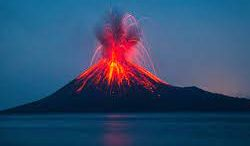
\includegraphics[width=100px]{4x1-relatifs/ex5.jpg}
  \end{figure}
\end{minipage}
\begin{minipage}[t]{0.75\textwidth}
  \textbf{3.} Le robot Curiosity relève les températures tous les jours. Aujourd'hui Il note un minimum a $-44 \degree C$. Il note un écart de température de $ 65\degree C$. La température maximum ne s'est pas enregistrée car il y avait une tempête de sable au moment de la transmission. Peut-on quand même connaître cette température maximale ?\\
  \Pointilles[3]
\end{minipage}

\Pointilles[2]

\begin{minipage}[t]{0.25\textwidth}
  \begin{figure}[H]
    \centering
    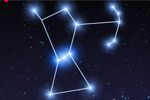
\includegraphics[width=100px]{4x1-relatifs/ex7.jpg}
  \end{figure}
\end{minipage}
  \begin{minipage}[t]{0.75\textwidth}
    \textbf{4.} Des scientifiques utilisent le télescope James Web (JWST) pour étudier la constellation d'Orion.
  \begin{itemize}
    \item La température de Rigel est de 11 300K.
    \item La température de notre Soleil est de 5800K.
    \item La température de Betelgeuse est de deux fois plus chaude que notre Soleil.
  \end{itemize}
  L'astronome Didier Queloz pense que Betelgeuse est plus froide que Rigel. A-t-il raison ? \\
\end{minipage}

\Pointilles[7]

\begin{minipage}[t]{0.25\textwidth}
  \begin{figure}[H]
    \centering
    
\includegraphics[width=100px]{4x1-relatifs/ex2.jpg}
  \end{figure}
\end{minipage}
\begin{minipage}[t]{0.75\textwidth}
  \textbf{5.} Dans FF7, votre personnage Cloud vient de subir une magie poison. Il s'affiche à l'écran -13HP toutes les 8 secondes. Sachant qu'il est au niveau 7 et possède 598HP, combien de temps peut-il survivre ?\\
  \Pointilles[6]
\end{minipage}

\Pointilles[3]

\begin{minipage}[t]{0.25\textwidth}
  \begin{figure}[H]
    \centering
    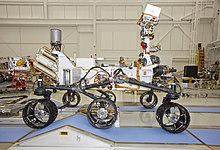
\includegraphics[width=100px]{4x1-relatifs/ex3.jpg}
  \end{figure}
\end{minipage}
\begin{minipage}[t]{0.75\textwidth}
  \textbf{6.} Dans Zelda, Link a le choix entre trois armes : 
  \begin{itemize}
    \item l'épée inflige 26 dégâts toutes les 6 secondes.
    \item La hache inflige 35 dégâts toutes les 10 secondes.
    \item La dague inflige 4 dégâts toutes les secondes.
  \end{itemize}
  Quelle arme est la plus efficace sur un temps de 1min ?\\
  \Pointilles[5]
\end{minipage}

\Pointilles[3]

\newpage

\textbf{Nom, Prénom :} \hspace{8cm} \textbf{Classe :} \hspace{3cm} \textbf{Date :}\\
\vspace{-0.8cm}
\begin{center}
  \textit{Je n'aime pas le travail, nul ne l'aime ; mais j'aime ce qui est dans le travail l'occasion de se découvrir soi-même.}  - \textbf{Joseph Conrad}
\end{center}
\vspace{-0.8cm}

\subsection*{Définitions}
  \begin{enumerate}
    \item[1.] Nombre négatif : \dotfill \\
    \Pointilles[1]
    \item[2.] Nombres opposés : \dotfill \\
    \Pointilles[1]
  \end{enumerate}

\subsection*{Exercice 1 - Calculer}

\begin{multicols}{3}\noindent
    \begin{enumerate}
        \item $70 \div 10 = \ldots\ldots$
        \item $10 \times \ldots\ldots = -100$
        \item $-3 \times 9 = \ldots\ldots$
        \item $-1 - \ldots\ldots = 1$
        \item $\ldots\ldots \times 4 = -8$
        \item $4 + \left( -1\right) = \ldots\ldots$
        \item $\ldots\ldots - \left( -8\right) = -2$
        \item $\ldots\ldots \times \left( -6\right) = 48$
        \item $13 - 4 = \ldots\ldots$
        \item $7 \div \left( -7\right) = \ldots\ldots$
        \item $6 \div 3 = \ldots\ldots$
        \item $-1 + 7 = \ldots\ldots$
        \item $1 - \left( -6\right) = \ldots\ldots$
        \item $-8 + 5 = \ldots\ldots$
        \item $\ldots\ldots \times 7 = -42$
        \item $5 - 7 = \ldots\ldots$
        \item $-50 \div \left( -10\right) = \ldots\ldots$
        \item $\ldots\ldots + \left( -9\right) = -14$
        \item $-6 + \left( -4\right) = \ldots\ldots$
        \item $40 \div \ldots\ldots = 4$
    \end{enumerate}
  \end{multicols}

\subsection*{Exercice 2 - signe d'un produit}

\begin{enumerate}
        \item $50 \times (-4)$ \dotfill
        \item $9 \times 6 \times 7$ \dotfill
        \item $-3 \times (-7) \times 4$ \dotfill
        \item $-11 \times (-7) \times -10 \times -1 \times 400$ \dotfill
        \item $2 \times -7 \times (-2) \times 5$ \dotfill
        \item $9 \times (-1) \times (-8)$ \dotfill
\end{enumerate}

\subsection*{Problèmes}

\begin{minipage}[t]{0.25\textwidth}
  \begin{figure}[H]
    \centering
    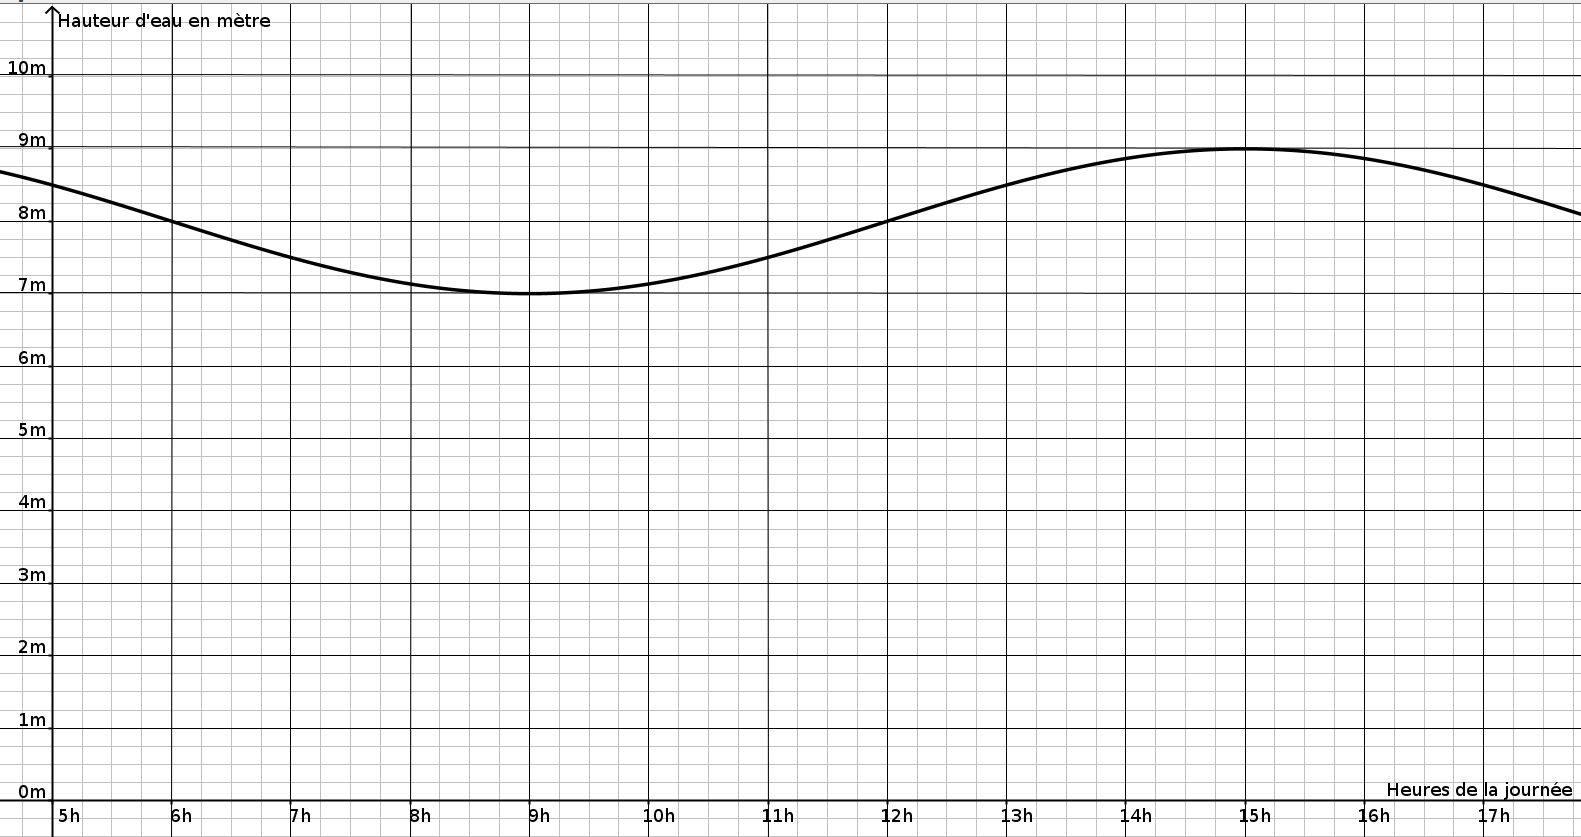
\includegraphics[width=100px]{4x1-relatifs/ex1.jpg}
  \end{figure}
\end{minipage}
\begin{minipage}[t]{0.75\textwidth}
\textbf{1.} Neil Armstrong de l'équipage d'Appolo 11 est sorti du module lunaire le 20 juillet 1969 pour faire le premier pas de l'Homme sur la Lune. La température sur la lune était de $-96 \degree C$. Sa combinaison était chauffée à une température de $16 \degree C$. 

Quelle était la différence de température entre l'intérieur et l'extérieur de sa combinaison ? \\
\Pointilles[6]
\end{minipage}

\begin{minipage}[t]{0.25\textwidth}
  \begin{figure}[H]
    \centering
    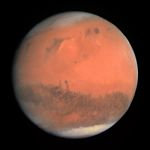
\includegraphics[width=100px]{4x1-relatifs/ex4.jpg}
  \end{figure}
\end{minipage}
\begin{minipage}[t]{0.75\textwidth}
  \textbf{2.} Sur Mars, la température le jour est de $28\degree C$ et la nuit de $-129\degree C$. Quelle est la différence de température entre le jour et la nuit ?\\
  \Pointilles[6]
\end{minipage}

\newpage

\begin{minipage}[t]{0.25\textwidth}
  \begin{figure}[H]
    \centering
    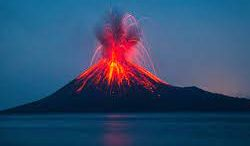
\includegraphics[width=100px]{4x1-relatifs/ex5.jpg}
  \end{figure}
\end{minipage}
\begin{minipage}[t]{0.75\textwidth}
  \textbf{3.} Le robot Curiosity relève les températures tous les jours. Aujourd'hui Il note un maximum de $14 \degree C$. Il note un écart de température de $ 65\degree C$. La température minimale ne s'est pas enregistrée car il y avait une tempête de sable au moment de la transmission. Peut-on quand même connaître cette température minimale ?\\
  \Pointilles[3]
\end{minipage}

\Pointilles[2]

\begin{minipage}[t]{0.25\textwidth}
  \begin{figure}[H]
    \centering
    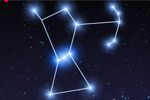
\includegraphics[width=100px]{4x1-relatifs/ex7.jpg}
  \end{figure}
\end{minipage}
  \begin{minipage}[t]{0.75\textwidth}
    \textbf{4.} Des scientifiques utilisent le télescope James Web (JWST) pour étudier la constellation d'Orion.
  \begin{itemize}
    \item La température de Rigel est de 11 300K.
    \item La température de notre Soleil est de 5800K.
    \item La température de Betelgeuse est de deux fois plus chaude que notre Soleil.
  \end{itemize}
  L'astronome Didier Queloz pense que Betelgeuse est plus chaude que Rigel. A-t-il raison ? \\
\end{minipage}

\Pointilles[7]

\begin{minipage}[t]{0.25\textwidth}
  \begin{figure}[H]
    \centering
    
\includegraphics[width=100px]{4x1-relatifs/ex2.jpg}
  \end{figure}
\end{minipage}
\begin{minipage}[t]{0.75\textwidth}
  \textbf{5.} Dans FF7, votre personnage Cloud vient de subir une magie poison. Il s'affiche à l'écran -13HP toutes les 8 secondes. Sachant qu'il est au niveau 7 et possède 698HP, combien de temps peut-il survivre ?\\
  \Pointilles[6]
\end{minipage}

\Pointilles[3]

\begin{minipage}[t]{0.25\textwidth}
  \begin{figure}[H]
    \centering
    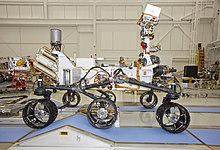
\includegraphics[width=100px]{4x1-relatifs/ex3.jpg}
  \end{figure}
\end{minipage}
\begin{minipage}[t]{0.75\textwidth}
  \textbf{6.} Dans Zelda, Link a le choix entre trois armes : 
  \begin{itemize}
    \item l'épée inflige 25 dégâts toutes les 6 secondes.
    \item La hache inflige 34 dégâts toutes les 10 secondes.
    \item La dague inflige 4 dégâts toutes les secondes.
  \end{itemize}
  Quelle arme est la plus efficace sur un temps de 1min ?\\
  \Pointilles[5]
\end{minipage}

\Pointilles[3]

\newpage

\end{document}